

\section{Relative calibration, flat field}% {\color{YellowGreen} Nico}}
\label{se:flatfields}

Absolute calibration requires known sources in the sky and the ability to
correct for atmospheric absorption. While absolute calibration of each KID also
\emph{de facto} provides relative calibration, the latter is interesting in
itself to characterize the instrument. We focus on this aspect in this section.\\

The dispersion of the detector responsivity across the field of view (\aka\ Flat
Fields) has been characterized in several ways:

% by estimating flat fields using the nominally
% focused \emph{beammap} scans described in Sect.~\ref{se:fp_reconstruction},
% because \bms\ are properly sampled and map high SNR point sources (see
% sect.~\ref{se:beammaps}). We have considered different kinds of flat fields:
\begin{itemize}
\item {\bf Main beam flat field.} This is the relative calibration of the KID main
  beam. It is the PSF response to a point source in the far field of the
  telescope. It is estimated per KID using \bms\ on bright sources that have the
  required sampling to give maps per individual KID (sect~\ref{se:beammaps}). We
  derive these ``gains'' $G_k$ as:
  \begin{equation}
    G_k = \frac{S_{th}(\nu_0)\, e^{-\tau/sin(\delta)}}{A_k}, 
  \end{equation}
  where $S_{th}(\nu_0)$ is the expected flux of the source integrated in the
  NIKA2 bandpasses and derived at the reference frequency $\nu_0$, 
  $\tau/sin(\delta)$ is the line-of-sight opacity measured using the
  \emph{skydip} method (sect.~\ref{se:opacities}) and $A_k$ is the
  amplitude of a Gaussian of fixed FWHM fitted from the detector $k$ map (as
  $\phi$ in Eq.~\ref{eq:flux_per_beam_def}).
\item {\bf Forward beam flat field:} the relative calibration of the response of
  each KID to the near field atmospheric background. It is estimated
  using the correlation factor of each detector TOI (apart from a bright source)
  to a median common mode estimated off-source (see sect.~\ref{se:toi_proc} for
  more details on common modes).
\end{itemize}

Figures \ref{fig:avg_mbff} and \ref{fig:avg_fbff} show the average main beam and
forward beam flat fields for the three arrays. These have been constructed by
combining the normalized flat fields of five \bms, which were
selected by thresholding the line-of-sight opacity measured in the 1\,mm band,
such as $\tau/sin(\delta) \leq 0.85$. The distributions for the average flat
fields are shown in the bottom panel of Fig.~\ref{fig:avg_mbff} and
\ref{fig:avg_fbff}.

We observe a sizable variation of the flat fields for A1 from the left-most side
to the right-most side of the FOV: this reveals a significant change of A1
detector responsivities depending on their position in the FOV. Namely, this
effect, the origin of which is under investigation, mainly impacts the left-most
third of the array, which will be referred to as the "shadow-zone''. This
variation of the flat field translates into a broadening of the
distribution. However, we verified that A1's flat field dispersions are in line
with the ones of A3 after the detectors within the shadow-zone were flagged out
using a crescent-shaped mask. The masked flat field distributions are shown in
green in Fig.~\ref{fig:avg_mbff} and \ref{fig:avg_fbff}, whereas shadow-zone
distributions are in red. In addition to the average flat fields, we further
characterize the flat fields for individual \bms. Fig.~\ref{fig:stddev_ff}
shows the dispersion of the flat fields for nine \bms\ using
either the whole FOV or masking the shadow-zone. The dispersion estimates for
this two cases are gathered in Table~\ref{tab:flatfields}.

\begin{table}[h]
\begin{center}
\begin{tabular}{|l|l|c|c|c|}
\hline
 Dispersion ($\%$)    & KID selection  &  A1 & A3  & A2 \\
\hline
Main beam flat field  & all the FOV           & $34.4 \pm 3.4$    & $15.5 \pm 1.4$  &  $13.2 \pm 1.7$  \\
                      & shadow-zone excluded  & $17.0 \pm 1.1$    & $14.2 \pm 1.2$  &  $12.8 \pm 1.3$\\
\hline
Forward beam flat field  & all the FOV           & $21.6 \pm 1.4$  & $10.1 \pm 1.7$  & $5.2 \pm 0.9$   \\
                         & shadow zone excluded  & $12.2 \pm 1.6$  & $10.1 \pm 2.1$  & $4.9 \pm 1.2$ \\
\hline
\end{tabular}
\caption[Flat field dispersions]{Average flat field dispersions in percent for
  nine \bms\ over all the FOV and after masking out the
  shadow-zone}
\end{center}
\label{tab:flatfields}
\end{table}


\begin{figure}[ht] 
\begin{center}
  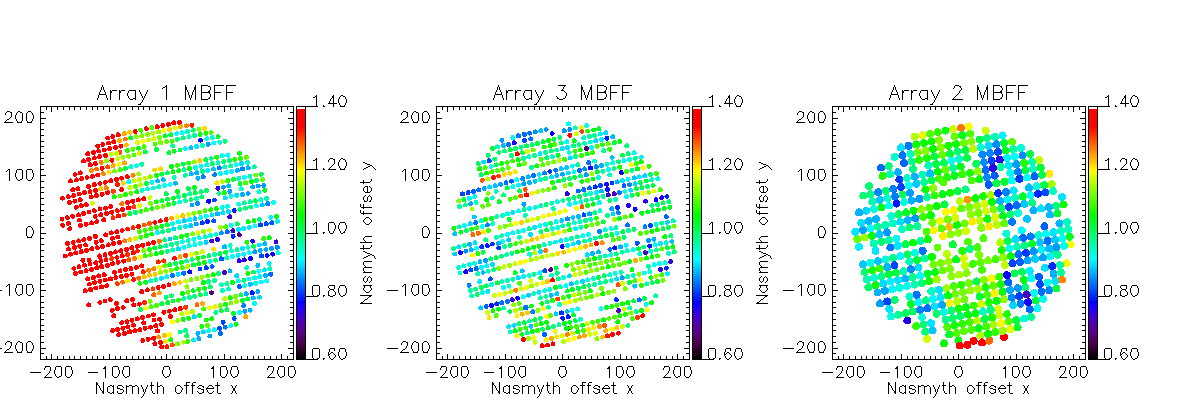
\includegraphics[width=0.95\textwidth]{Figures/FlatFields/Average_main_beam_flat_field_N2R9_10.png}
  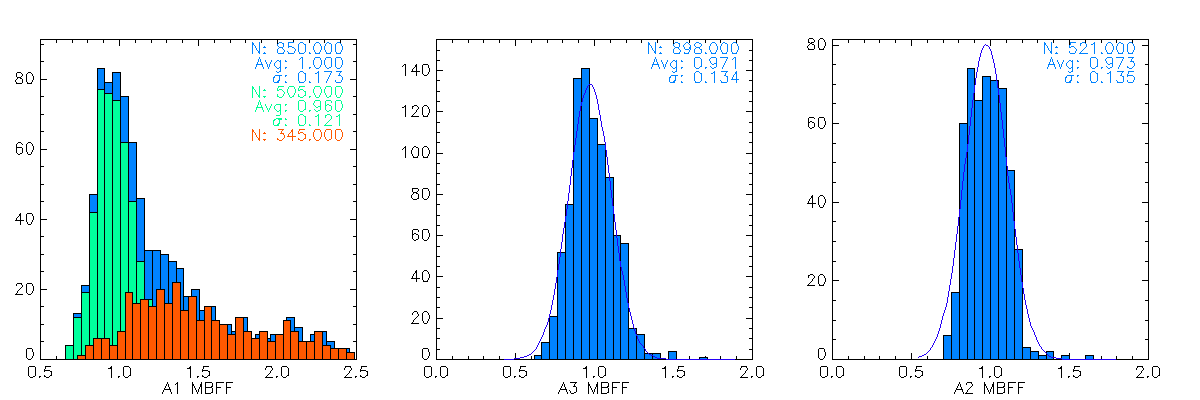
\includegraphics[width=0.8\textwidth]{Figures/FlatFields/Histo_average_main_beam_flat_field_N2R9_10.png}
\caption[Average main beam flat fields]{Average main beam flat fields
  obtained by combining the normalized flat fields of five
  \bm\ scans. The top row plots show the average flat fields of Array
  1, 3 and 2 in Nasmyth coordinates, and the bottom plots
  show the average flat field distributions using all KIDs (blue),
  using Array 1 KIDs that are positioned out of the shadow zone
  (green) and using Array 1 KIDs inside the shadow zone, which is
  defined in the text.}
 \label{fig:avg_mbff}
\end{center}
\end{figure}

\begin{figure}[ht] 
\begin{center}
  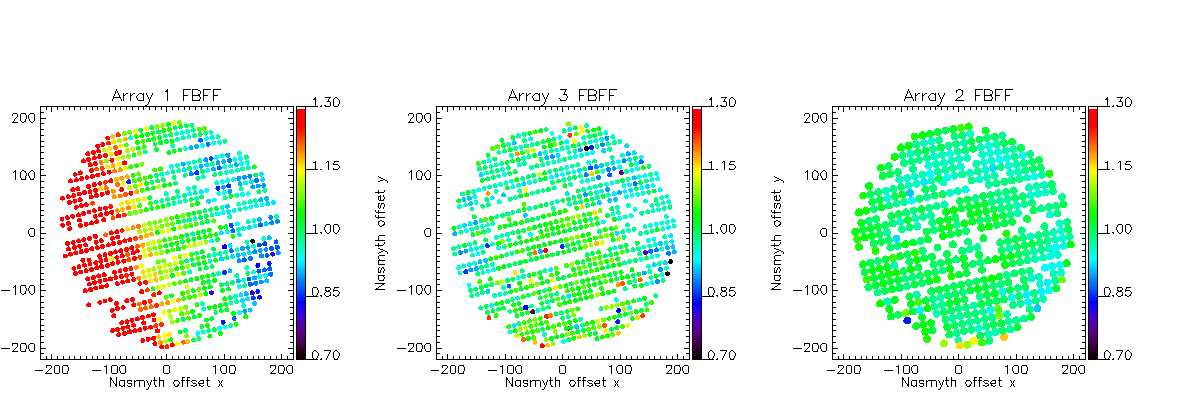
\includegraphics[width=0.95\textwidth]{Figures/FlatFields/Average_near_beam_flat_field_N2R9_10.png}
  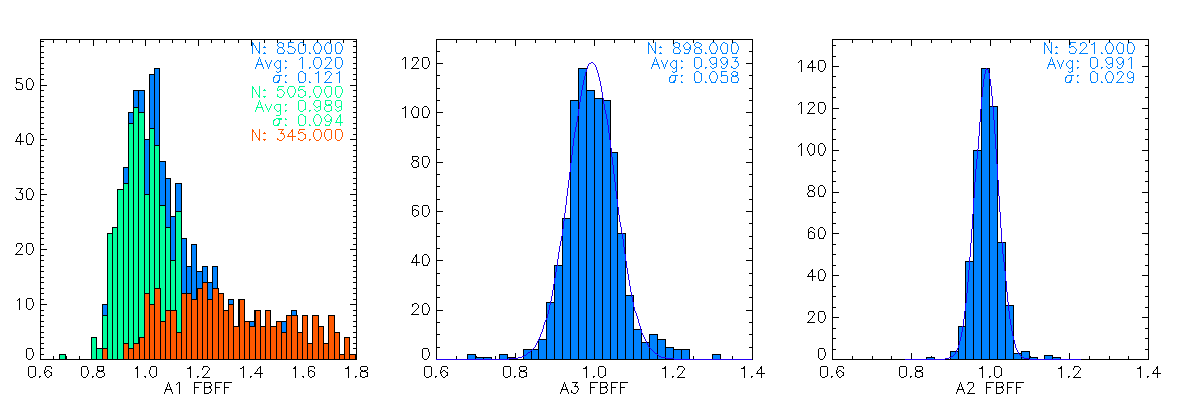
\includegraphics[width=0.8\textwidth]{Figures/FlatFields/Histo_average_near_beam_flat_field_N2R9_10.png}
\caption[Average forward efficiency flat fields]{Average forward efficiency flat field for array 1, 3 and
  2. Same legend as Fig.~\ref{fig:avg_mbff}}
 \label{fig:avg_fbff}
\end{center}
\end{figure}

\begin{figure}[ht] 
\begin{center}
  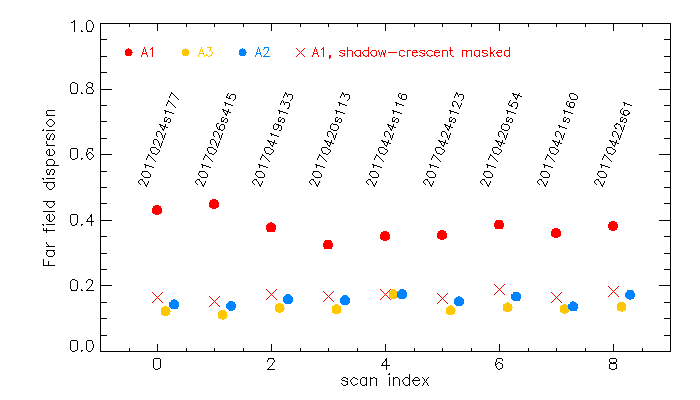
\includegraphics[width=0.6\textwidth]{Figures/FlatFields/Dispersion_main_beam_flat_field_N2R9_10_.png}
  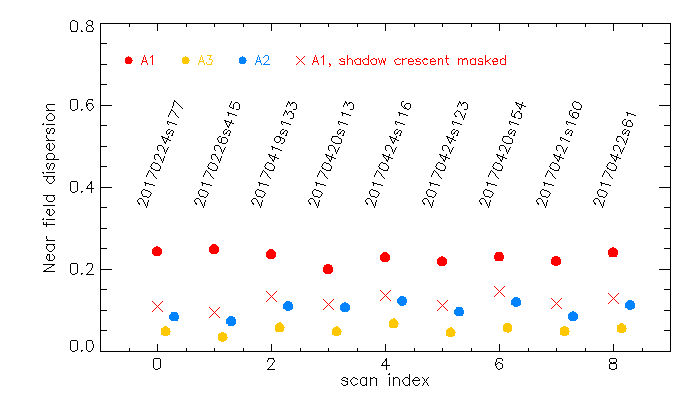
\includegraphics[width=0.6\textwidth]{Figures/FlatFields/Dispersion_forward_beam_flat_field_N2R9_10_.png}
\caption[Dispersion of the flat field for nine \bms.]{The RMS
  dispersion of the normalised main beam flat field (upper panel) and forward beam flat
  field (lower panel) are shown using all valid KIDs of Array 1 (red circles),
  Array 3 (orange circles) and Array 2 (blue circles), and using the KIDs
  located outside the Array 1 "shadow area'', which was discarded using a left
  crescent-shaped mask (red crosses).}
 \label{fig:stddev_ff}
\end{center}
\end{figure}
